% !TeX spellcheck = en_US
\documentclass{beamer}
\usepackage[latin1]{inputenc}
\usepackage{dsfont}
\usepackage{color}
\usepackage{tabularx}
\usepackage{amssymb}

% % % % % FRAME STYLE

\setbeamertemplate{navigation symbols}{}
\setbeamertemplate{frametitle}{\vspace{10mm}\hspace{0mm}\insertframetitle}
\setbeamertemplate{footline}{\hfill\insertframenumber/\inserttotalframenumber\hspace{5mm}\vspace{5mm}}

\usefonttheme{structurebold}
\usecolortheme{dove}

\AtBeginSection[]
{
	\begin{frame}
		\frametitle{Agenda}
		\tableofcontents[currentsection]
	\end{frame}
}

% % % % % CUSTOM COMMANDS
\newcommand{\Empty}{\mbox{$\varnothing$}}
\newcommand{\NotEmpty}{\mbox{$\neg\varnothing$}}

% % % % % FRAMES

\begin{document}

	\title{Qualitative Spatial Reasoning over Line-Region Relations}
	\author{Leena and Sibel}
	\date{Knowledge Representation\\Seminar Presentation}

	
	\begin{frame}
		\titlepage
	\end{frame}
	
	\section{Motivation}
	
	
	\section{Definitions and Formalisms}
	
	\subsection{Lines and Regions}
	\subsection{Topological Parts of an Object}
	\subsection{9-Intersection}
	
	\section{Models of Conceptual Neighborhoods}
	
	\subsection{Snapshot Model}
	
	\begin{frame}{Snapshot Model}
		
	\end{frame}
	
	\begin{frame}{Resulting Neighborhood Graph}
		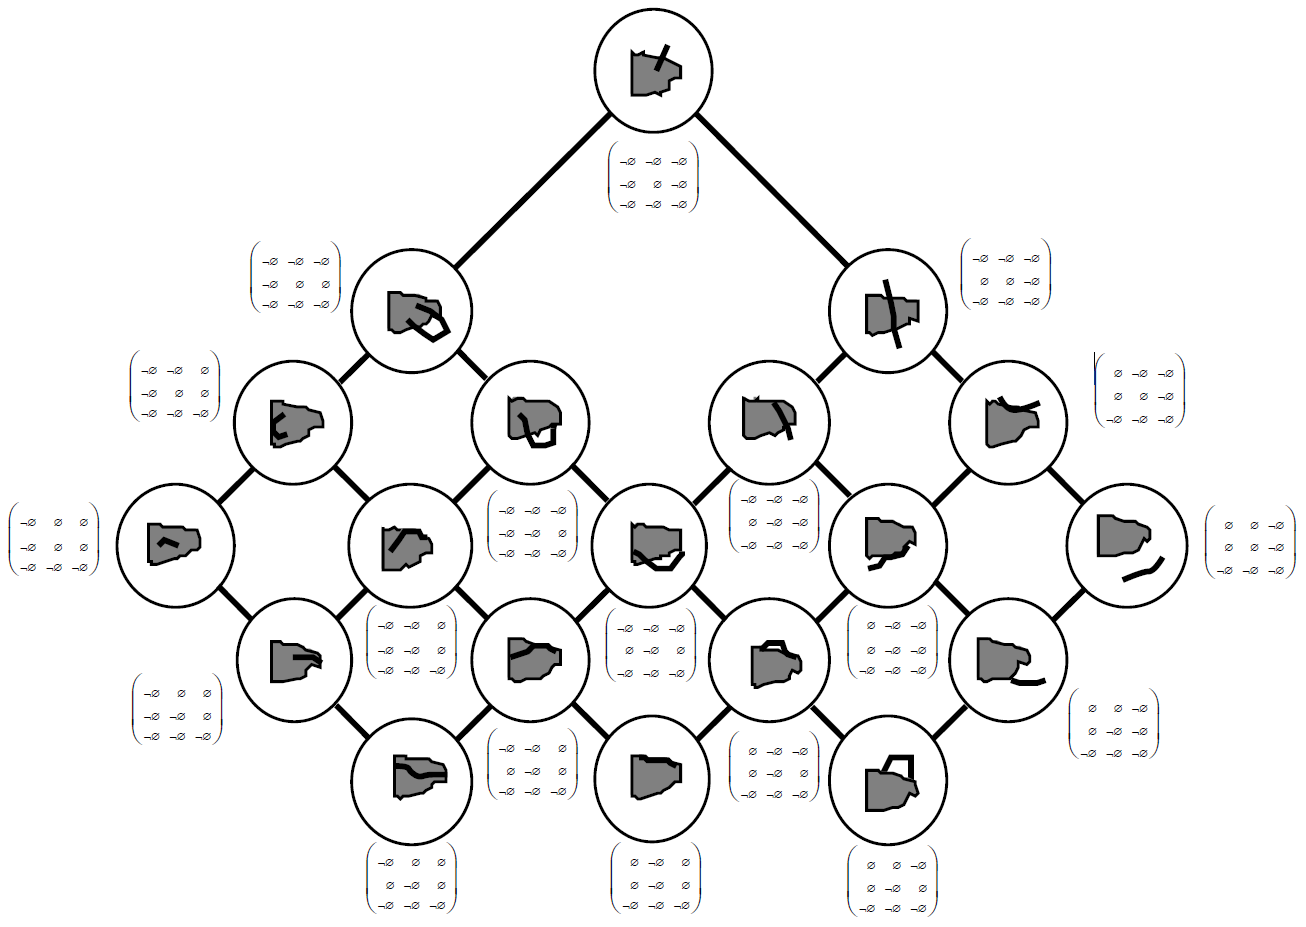
\includegraphics[width=\textwidth]{images/snapshot_model_neighborhood_graph.png}
	\end{frame}
	
	\subsection{Smooth-Transition Model}
	
	\begin{frame}{Smooth-Transition Model}
		\begin{block}{Smooth Transition}
			infinitesimally small deformation that changes the topological relation
		\end{block}
		\begin{block}{Formalization based on} for lines and regions, such changes may be thought of as
			\begin{enumerate}
				\item Moving a line's boundary node from a region part into an adjacent part of the region.
				
				\item Moving a line's interior partially from a region part into an adjacent part of the region.
			\end{enumerate}
		a total of 4? rules
		Define extent of a part i
		\end{block}
	\end{frame}
	
	% Draw 9-intersection model on the board for reference
	
	\begin{frame}{Moving the Line's Boundaries}
		\begin{block}{Rule 1}
			If the line's two boundaries intersect with the same region part, then extend the intersection to either of the adjacent region parts.
		\end{block}
		
		\begin{block}{Formalization}
			\centering $ \#M[\delta, \_] = 1 \Rightarrow
			\forall i (M[\delta, i] = \NotEmpty):
				M_{N}[\delta, \text{adjacent}(i)] := \NotEmpty $
		\end{block}
		
		\begin{block}{Example}
			%Moving one boundary of a line into an adjacent part of the region.
			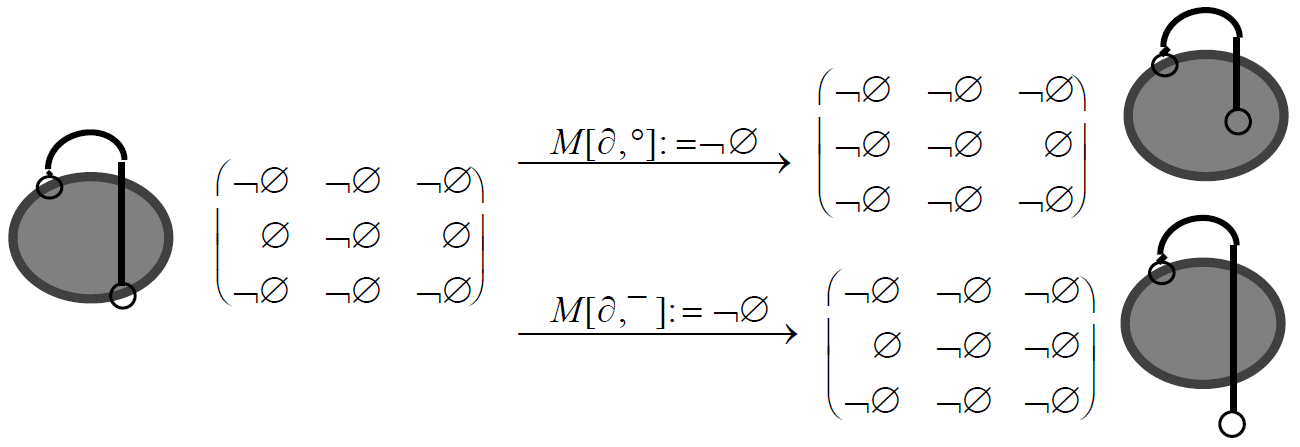
\includegraphics[width=\textwidth]{images/smooth_transitions_example_a.png}
		\end{block}
	\end{frame}
	
	\begin{frame}{Moving the Line's Boundaries}
		\begin{block}{Rule 2}
			If the line's two boundaries intersect with two different region parts then move either intersection to the adjacent region part.
		\end{block}
		
		\begin{block}{Formalization}
			\centering $ \#M[\delta,\_] = 2 \Rightarrow
			\forall i (M[\delta, i] = \NotEmpty):
				M_{N}[\delta, i] := \Empty \text{ \textbf{and} }
				M_{N}[\delta, \text{adjacent}(i)] := \NotEmpty $
		\end{block}
		
		\begin{block}{Example}
			%Moving either boundary into an adjacent region part.
			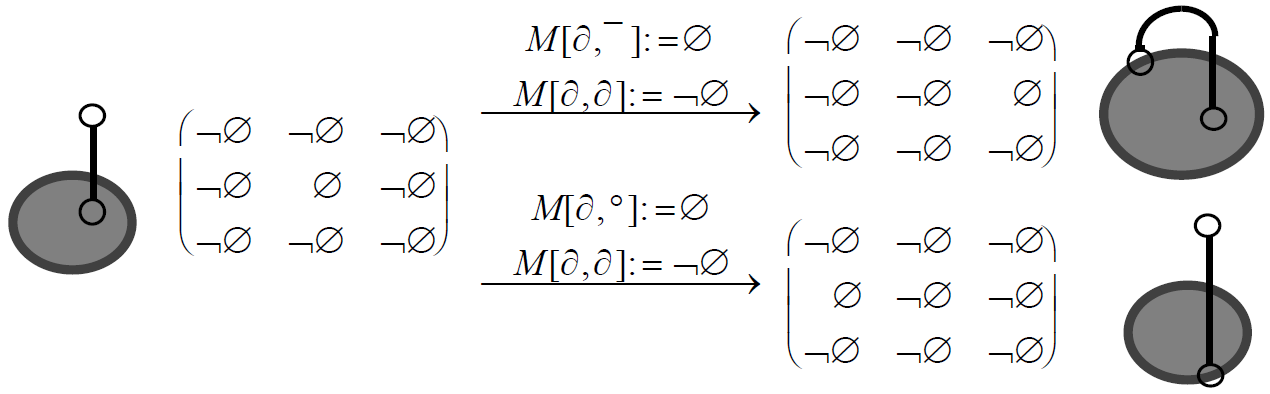
\includegraphics[width=\textwidth]{images/smooth_transitions_example_b.png}
		\end{block}
	\end{frame}
	
	\begin{frame}{Moving the Line's Interior}
		\begin{block}{Rule 1}
			Extend the line's interior-intersection to either of the adjacent region parts.
		\end{block}
		
		\begin{block}{Formalization}
			\centering $ \forall i (M[�, i] = \NotEmpty):
			M_{N}[�, \text{adjacent}(i)] := \NotEmpty $
		\end{block}
		
		\begin{block}{Example}
			%Moving the line's interior into an adjacent part of the region.
			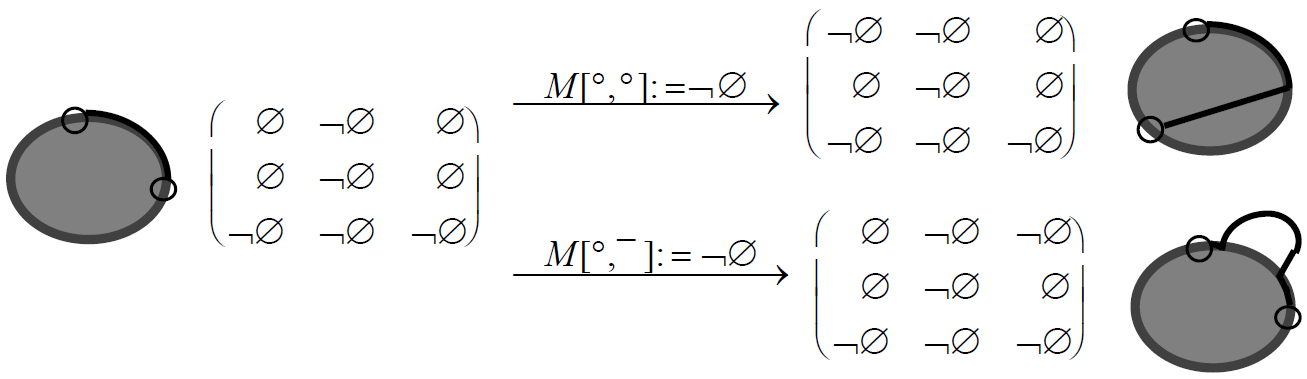
\includegraphics[width=\textwidth]{images/smooth_transitions_example_c.png}
		\end{block}
	\end{frame}
	
	\begin{frame}{Moving the Line's Interior}
		\begin{block}{Rule 2}
			Reduce the line's interior intersection on either of the adjacent region parts.
		\end{block}
		
		\begin{block}{Formalization}
			\centering
			$ \#M[�, \_] = 2 \Rightarrow
			\forall i (M[�, i] = \NotEmpty):
			M_{N}[�, i] := \Empty $
			$ \#M[�, \_] = 3 \Rightarrow
			\forall i (i \neq \delta):
			M_{N}[�, i] := \Empty $
		\end{block}
		
		\begin{block}{Example}
			%Moving the line's interior out of a part of the region.
			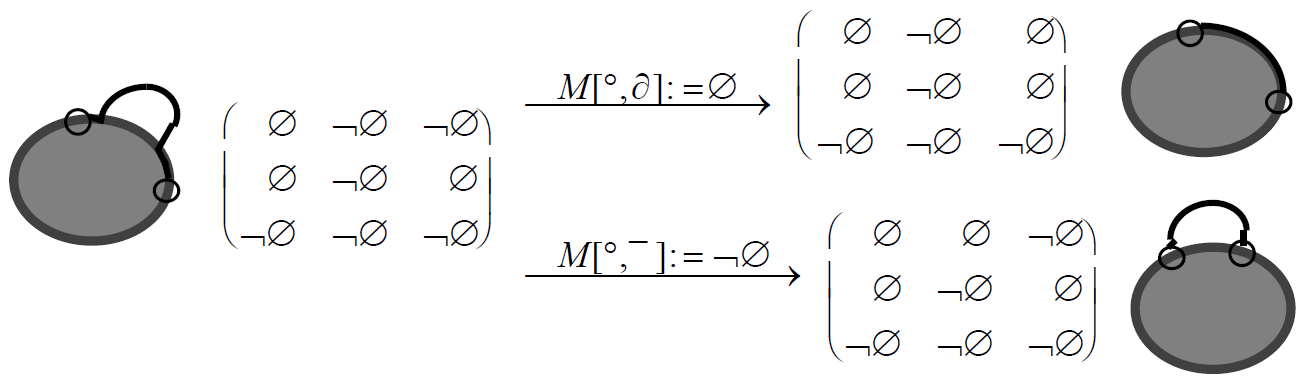
\includegraphics[width=\textwidth]{images/smooth_transitions_example_d.png}
		\end{block}
	\end{frame}
	
	\begin{frame}{Consistency Constraints}
		\begin{enumerate}
			\item If the line's interior intersects with the region's interior \textit{and} exterior, then the line's interior must also intersect with the region's boundary.
			\begin{center}
				$ M[�,�] = \NotEmpty \text{and} M[�,^{-}] = \NotEmpty \Rightarrow M[�,\delta] := \NotEmpty $
			\end{center}
			
			\item If the line's boundary intersects with the region's interior (exterior) then the line's interior must intersect with the region's interior (exterior) as well.
			\begin{center}
				$ M[\delta, �] = \NotEmpty M[�,�] := \NotEmpty $ \\
				$ M[\delta, ^{-}] = \NotEmpty M[�,^{-}] := \NotEmpty $
			\end{center}
		\end{enumerate}

	\end{frame}
	
	% NOTES:
	% The separate moves of the line's interior and boundaries are atomic operations that do not account for some of the properties of the objects and their embedding space and, therefore, may generate inconsistent 9-intersections for configurations that cannot be realized. In order to maintain connectivity among the line's boundaries and interior, it is necessary to assure the following \textbf{consistency constraint}: [1]. Likewise, in order to preserve the continuous-space property of $\mathcal{R}^{2}$, the following consistency constraint must be fulfilled: [2].
	
	\begin{frame}{Resulting Neighborhood Graph}
		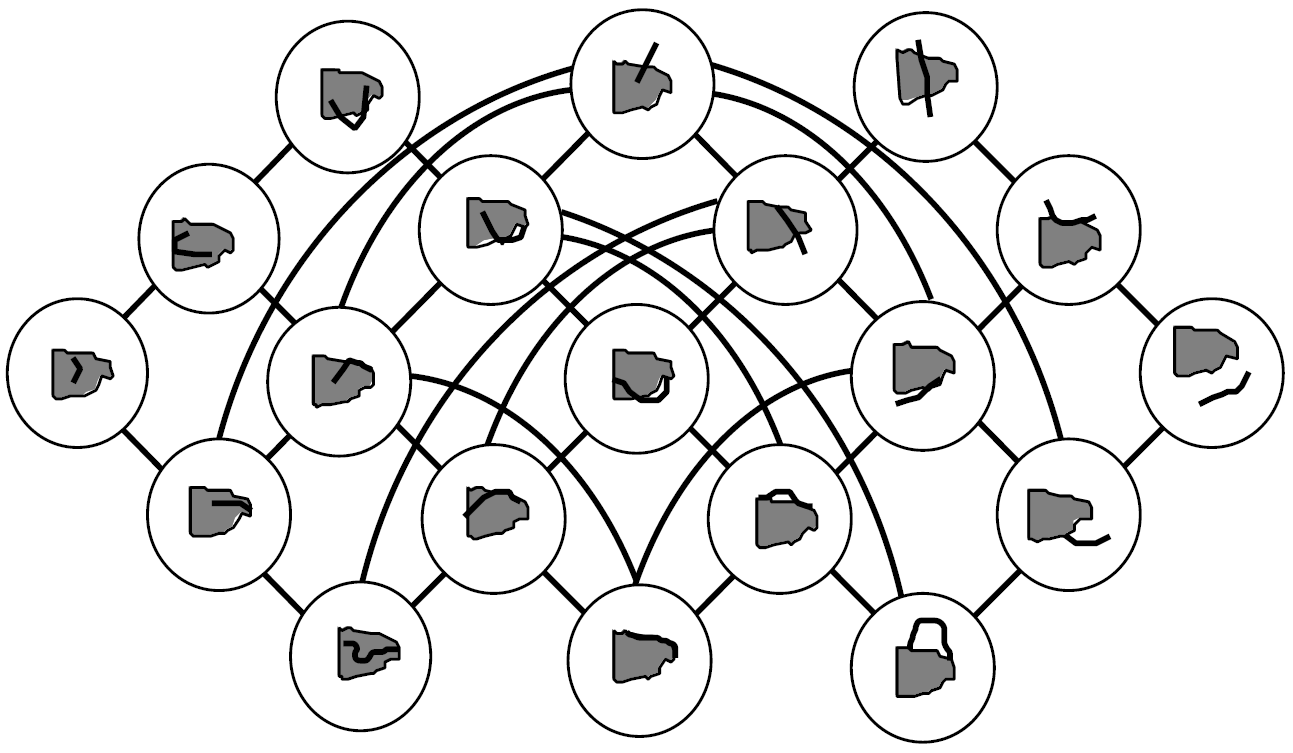
\includegraphics[width=\textwidth]{images/smooth_transitions_neighborhood_graph.png}
	\end{frame}
	
	% NOTES:
	% This graph resembles in most of its structure and properties the snapshot neighborhood graph. The difference between the two graphs are
	%\begin{itemize}
	%	\item the way in which conceptual neighbors are connected at the top,
	%	\item the additional links that run across the smooth transition graph.
	%\end{itemize}
	
	
	\section{Evaluation}
	
	\section{Conclusion}

	
	
	\begin{frame}{References}  
		\begin{thebibliography}{10}    
%			\beamertemplatebookbibitems
%			\bibitem{Diekert2013}
%			V.~Diekert, M.~Kufleitner, G.~Rosenberger.
%			\newblock {\em Diskrete Algebraische Methoden}. (Abschnitt 7.6)
%			\newblock Walter de Gruyter, 2013.
%			\beamertemplatearticlebibitems
%			\bibitem{Heller2008}
%			A.~Heller.
%			\newblock Ein Entscheidungsverfahren f�r die Presburger Arithmetik.
%			\newblock https://www4.in.tum.de/lehre/vorlesungen/perlen/SS08/\\Unterlagen/Presburger.pdf.
		\end{thebibliography}
	\end{frame}
\end{document}